\documentclass[conference]{IEEEtran}
\IEEEoverridecommandlockouts
\usepackage[T1]{fontenc}
\usepackage[utf8]{inputenc}
\usepackage[turkish]{babel}
\usepackage{cite}
\usepackage{amsmath,amssymb,amsfonts}
\usepackage{graphicx}
\usepackage{booktabs}
\usepackage{siunitx}
\usepackage{xcolor}
\usepackage[hidelinks]{hyperref}

\title{12 Kanall\i\ EKG S\i n\i fland\i rmas\i nda Belirleyici Ad\i m: \\
       Anti-Aliasing'li Alt\"{o}rnekleme ile Chapman--Shaoxing \"{u}zerinde \\
       Temel 1D-CNN ile \SI{88,43}{\percent}'ten \SI{97,34}{\percent}'e}

\author{\IEEEauthorblockN{Elaman Nazarkulov}
\IEEEauthorblockA{Bilgisayar M\"{u}hendisli\u{g}i B\"{o}l\"{u}m\"{u} \\
K\i rg\i z--T\"{u}rk Manas \"{U}niversitesi \\
Bi\c{s}kek, K\i rg\i zistan \\
elaman.job@gmail.com}}

\begin{document}
\maketitle

\begin{abstract}
Otomatik 12 kanall\i\ elektrokardiyogram (EKG) s\i n\i fland\i rmas\i\
geleneksel olarak kanal ba\c{s}\i na \num{5000} \"{o}rnekten olu\c{s}an
ham \SI{500}{\hertz}\,$\times$\,\SI{10}{\second} sinyali \"{u}zerinde
yap\i l\i r. Bu \c{c}al\i\c{s}mada, s\"{o}z konusu varsay\i lan giri\c{s}
uzunlu\u{g}unun, Chapman--Shaoxing veri seti (\num{45152} kay\i t,
\num{78} \c{c}oklu-etiket s\i n\i f\i ) \"{u}zerinde temel bir 1B
evri\c{s}imli sinir a\u{g}\i\ (1D-CNN) i\c{c}in
\emph{belirleyici} bir tasar\i m se\c{c}imi oldu\u{g}u --- n\"{o}tr bir
varsay\i lan olmad\i\u{g}\i\ --- g\"{o}sterilmi\c{s}tir. Giri\c{s}
sinyalinin \texttt{scipy.signal.decimate} ile \num{500} \"{o}rne\u{g}e
(etkin \SI{50}{\hertz}) anti-aliasing'li alt\"{o}rneklenmesi, test
do\u{g}rulu\u{g}unu \SI{88,43}{\percent}'ten \SI{97,34}{\percent}'e,
makro-$F_1$ de\u{g}erini \num{0,8713}'ten \num{0,9737}'ye
y\"{u}kseltirken, tekil \"{o}rnek \"{u}zerinde \c{c}\i kar\i m s\"{u}resini
\SI{89,88}{\milli\second}'den \SI{27,20}{\milli\second}'ye
indirmektedir. Temel modelde $F_1<0,60$ olan on bir ba\c{s}ar\i s\i z
s\i n\i f (en k\"{o}t\"{u} durum: Sol Ventrik\"{u}ler Hipertrofi,
$F_1=\num{0,022}$) tek tip bi\c{c}imde $F_1\geq \num{0,95}$ d\"{u}zeyine
\c{c}\i kmaktad\i r. Bulgu, \emph{geometrik de\u{g}i\c{s}mezlik
arg\"{u}man\i} \c{c}er\c{c}evesinde de\u{g}erlendirilmi\c{s}tir: EKG'nin
tan\i sal i\c{c}eri\u{g}i, at\i m ba\c{s}\i na P, Q, R, S, T olmak \"{u}zere
yakla\c{s}\i k \num{60} referans nokta i\c{c}eren seyrek bir yap\i da
yo\u{g}unla\c{s}\i r ve Chebyshev-I anti-aliasing filtresi bu noktalar\i\
$\pm\SI{10}{\milli\second}$ hassasiyetinde korur. Girdinin
\num{5000}\,$\rightarrow$\,\num{500} \"{o}rne\u{g}e indirgenmesi,
referans nokta yo\u{g}unlu\u{g}unu 10$\times$ art\i r\i r ve CNN'in
etkin al\i c\i\ alan\i n\i n t\"{u}m \SI{10}{\second} pencereyi
kapsamas\i n\i\ sa\u{g}lar. \c{C}al\i\c{s}ma, giri\c{s} uzunlu\u{g}unun
EKG k\i yaslama \c{c}al\i\c{s}malar\i nda yeterince raporlanmam\i\c{s}
bir tasar\i m de\u{g}i\c{s}keni oldu\u{g}unu ve son d\"{o}nem
literat\"{u}rdeki y\"{u}ksek do\u{g}ruluk iddialar\i n\i n k\i smen mimari
iyile\c{s}tirmelerden de\u{g}il, giri\c{s} uzunlu\u{g}u optimizasyonundan
kaynaklanabilece\u{g}ini savunmaktad\i r.
\end{abstract}

\begin{IEEEkeywords}
elektrokardiyogram, 12 kanall\i\ EKG, derin \"{o}\u{g}renme, 1B
evri\c{s}imli sinir a\u{g}\i, anti-aliasing'li alt\"{o}rnekleme,
\c{c}oklu-etiket s\i n\i fland\i rma, sinyal \"{o}n i\c{s}leme,
referans noktalar, geometrik de\u{g}i\c{s}mezlik.
\end{IEEEkeywords}

\section{Giri\c{s}}
Derin evri\c{s}imli sinir a\u{g}lar\i, 12 kanall\i\ EKG yorumlamas\i nda
art\i k kardiyolog d\"{u}zeyinde performans
sa\u{g}lamaktad\i r~\cite{rajpurkar2017,hannun2019,strodthoff2020}.
Standart giri\c{s} temsili, sinyali al\i nd\i\u{g}\i\ \"{o}rnekleme h\i z\i nda
(\c{c}o\u{g}u zaman \SI{500}{\hertz}) modele besler ve
\SI{10}{\second}'lik bir segment i\c{c}in kanal ba\c{s}\i na \num{5000}
\"{o}rnek \"{u}retir. Bu se\c{c}im nadiren sorgulan\i r: veri
art\i rma~\cite{iwana2021,wang2020}, destek-d\"{u}\u{g}\"{u}m
interpolasyonu~\cite{chen2021,xu2022} ve hibrit yinelemeli ya da
attention tabanl\i\ mimariler~\cite{oh2018,strodthoff2020} hep bu sabit
giri\c{s} \"{u}zerinde de\u{g}erlendirilir.

\"{O}nceki tez d\"{o}nemimizde Chapman--Shaoxing~\cite{zheng2020} \"{u}zerinde
e\u{g}itilen temel 1D-CNN, yaln\i zca \SI{88,43}{\percent} test
do\u{g}rulu\u{g}u ve \num{0,8713} makro-$F_1$ de\u{g}erine ula\c{s}m\i\c{s};
\num{78} etiketten \num{11}'i $F_1<0,60$ d\"{u}zeyinde
\c{c}\"{o}km\"{u}\c{s}t\"{u}r. Do\u{g}al refleks, attention katmanlar\i,
yinelemeli kodlay\i c\i lar, focal loss~\cite{lin2017} ve etiket-taksonomi
temizli\u{g}i planlamak olmu\c{s}tur. Bu makale ise tersi bir hipotezi
test etmektedir: \num{5000} \"{o}rnekli giri\c{s}, CNN'in yararl\i\ bir
\c{s}ekilde kullanabilece\u{g}inden daha fazla zamansal art\i kl\i k
ta\c{s}\i maktad\i r ve tek sat\i rl\i k bir \"{o}n i\c{s}leme
de\u{g}i\c{s}ikli\u{g}i --- \num{500} \"{o}rne\u{g}e anti-aliasing'li
alt\"{o}rnekleme --- t\"{u}m tan\i sal a\c{c}\i dan ilgili \"{o}zellikleri
korurken gradyan sinyalini bu \"{o}zellikler \"{u}zerinde
yo\u{g}unla\c{s}t\i r\i r.

\noindent\textbf{Katk\i lar.}
\begin{enumerate}
  \item Chapman--Shaoxing \"{u}zerinde, \emph{ayn\i} model, art\i rma,
        optimizasyon, seed ve ay\i rma ile giri\c{s} uzunluklar\i\
        $\{\num{5000}, \num{1000}, \num{500}\}$'\"{u}n kontroll\"{u}
        kar\c{s}\i la\c{s}t\i rmas\i.
  \item Giri\c{s}in 10$\times$ alt\"{o}rneklenmesinin, temel 1D-CNN ile
        literat\"{u}rde s\i k\c{c}a al\i nt\i lanan attention-hibrit
        \SI{94,8}{\percent} hedefi~\cite{oh2018} aras\i ndaki bo\c{s}lu\u{g}un
        b\"{u}y\"{u}k k\i sm\i ndan sorumlu oldu\u{g}una dair kan\i t.
  \item On bir ba\c{s}ar\i s\i z s\i n\i f\i n ($F_1<0,60$) tamam\i n\i n
        modelde, kay\i pta veya art\i rma re\c{c}etesinde hi\c{c}bir
        de\u{g}i\c{s}iklik yap\i lmadan $F_1\geq\num{0,95}$'a d\"{o}nd\"{u}\u{g}\"{u}n\"{u}
        g\"{o}steren s\i n\i f baz\i nda iyile\c{s}me analizi ve bunun
        nedenini a\c{c}\i klayan geometrik-de\u{g}i\c{s}mezlik
        arg\"{u}man\i.
\end{enumerate}

\section{\.{I}lgili \c{C}al\i\c{s}malar}
\textbf{Derin EKG s\i n\i fland\i rmas\i.}
Rajpurkar~ve~ark.~\cite{rajpurkar2017} ve
Hannun~ve~ark.~\cite{hannun2019} \num{91232} ambulatuvar EKG \"{u}zerinde
e\u{g}ittikleri derin CNN'lerle 12--14 ritm s\i n\i f\i nda kardiyolog
seviyesinde performans elde etmi\c{s}lerdir.
Strodthoff~ve~ark.~\cite{strodthoff2020} PTB-XL~\cite{wagner2020}
\"{u}zerinde CNN, RNN ve Transformer modellerini kar\c{s}\i la\c{s}t\i rmak
i\c{c}in kayna\u{g}a duyarl\i\ olarak \SI{100}{\hertz} (\num{1000} \"{o}rnek)
girdi kullanm\i\c{s} ve makro-AUC \num{0,925} bildirmi\c{s}lerdir; bu,
\SI{500}{\hertz}'in zorunlu olmad\i\u{g}\i\ y\"{o}n\"{u}nde sessiz bir ipucudur.
Oh~ve~ark.~\cite{oh2018} CNN--LSTM hibrit modelle de\u{g}i\c{s}ken-uzunlukta
at\i mlarda \SI{94,8}{\percent} do\u{g}ruluk bildirmi\c{s}; bu rakam,
\"{o}nceki d\"{o}nem tez raporumuzun a\c{c}\i k hedefiydi.

\textbf{Art\i rma ve dengesizlik.}
Iwana~ve~Uchida~\cite{iwana2021} zaman serisi art\i rma tekniklerini
kapsaml\i\ olarak incelemi\c{s}tir. GAN tabanl\i\ \"{u}retim~\cite{wang2020}
ve fiducial-noktada destek-y\"{o}nl\"{u} interpolasyon~\cite{chen2021,xu2022}
EKG-\"{o}zg\"{u} re\c{c}eteler aras\i nda \"{o}ne \c{c}\i kar. Focal
loss~\cite{lin2017} ve ters-frekans a\u{g}\i rl\i kland\i rma s\i n\i f
dengesizli\u{g}ine standart yan\i tlard\i r.

\textbf{\"{O}rnekleme h\i z\i\ se\c{c}imi.}
Mimari ve art\i rma \"{u}zerine kapsaml\i\ ablation \c{c}al\i\c{s}malar\i na
ra\u{g}men, giri\c{s} \"{o}rnekleme h\i z\i\ at\i fta bulunulan \c{c}al\i\c{s}malarda bir
kez yap\i land\i r\i l\i p tekrar ele al\i nmamaktad\i r. Bilgimiz dahilinde,
\"{o}nceki hi\c{c}bir b\"{u}y\"{u}k \"{o}l\c{c}ekli 12 kanall\i\ EKG \c{c}al\i\c{s}mas\i\
giri\c{s}-uzunlu\u{g}u ablation'\i n\i\ ana sonu\c{c} olarak raporlamam\i\c{s}t\i r.

\section{Y\"{o}ntem}
\subsection{Veri seti}
Chapman--Shaoxing 12 kanall\i\ EKG veritaban\i n\i\ kullan\i yoruz~\cite{zheng2020}:
\SI{500}{\hertz}'te \num{45152} kay\i t, her biri \SI{10}{\second}, \num{78}
\c{c}oklu-etiket tan\i sal kategori ile annotate edilmi\c{s}tir. Veri seti normal
sin\"{u}s ritmi, atriyal flatter, atriyal fibrilasyon, sin\"{u}s
bradikardi/ta\c{s}ikardi, AV blok, ventrik\"{u}ler ekstrasistol, dal blokaj\i\
ve \num{70}'ten fazla nadir alt-kategoriyi kapsar. S\i n\i f
dengesizli\u{g}i ciddidir: en s\i k g\"{o}r\"{u}len d\"{o}rt s\i n\i f ham
kay\i tlar\i n \num{34000}'den fazlas\i n\i\ olu\c{s}tururken, \num{30}+ s\i n\i f
\num{50}'den az \"{o}rne\u{g}e sahiptir.

\subsection{\"{O}n i\c{s}leme hatt\i}
T\"{u}m konfig\"{u}rasyonlarda ayn\i\ \"{o}n i\c{s}leme uygulan\i r:
\begin{enumerate}
  \item sinc interpolasyon ile \SI{500}{\hertz}'e yeniden \"{o}rnekleme;
  \item \SIrange{0,5}{150}{\hertz} bant ge\c{c}iren filtre (Butterworth, 4. derece) ve
        \c{s}ebeke giri\c{s}imi i\c{c}in \SI{50}{\hertz} \c{c}entik filtre;
  \item taban kayma giderimi i\c{c}in \SI{0,5}{\hertz} y\"{u}ksek ge\c{c}iren filtre;
  \item kanal-ba\c{s}\i na $Z$-skor normalle\c{s}tirme ve $\pm 3\sigma$ k\i rpma;
  \item sabit \SI{10}{\second} segmentasyon ($[12 \times \num{5000}]$);
  \item Sinyal Kalite \.{I}ndeksi filtresi SQI${} \geq \num{0,85}$;
  \item \emph{alt\"{o}rnekleme ad\i m\i\ (bu makale)}: yaln\i zca temel
        olmayan konfig\"{u}rasyonlarda uygulan\i r,
        bkz.\ B\"{o}l\"{u}m~\ref{sec:dec};
  \item destek-d\"{u}\u{g}\"{u}m art\i rma~\cite{xu2022}: yayg\i n s\i n\i flar
        i\c{c}in 3$\times$, nadir s\i n\i flar i\c{c}in 10$\times$, hedef
        s\i n\i f ba\c{s}\i na \num{4500} \"{o}rnek.
\end{enumerate}
T\"{u}m konfig\"{u}rasyonlarda tek bir seed ile sabitlenmi\c{s} 68/12/20
e\u{g}itim/do\u{g}rulama/test ay\i rmas\i\ kullan\i lm\i\c{s}t\i r.

\subsection{Anti-aliasing'li alt\"{o}rnekleme}
\label{sec:dec}
$x\in\mathbb{R}^{12\times N}$, $N=\num{5000}$ olmak \"{u}zere, alt\"{o}rnekleme
ad\i m\i\ \texttt{scipy.signal.decimate}~\cite{scipy2020} \"{u}zerine tek bir
\c{c}a\u{g}r\i d\i r:
\begin{equation}
x' = \operatorname{decimate}\!\bigl(x,\, q,\,
   \text{ftype}=\text{`iir'},\, n=8,\,
   \text{zero\_phase}=\text{True}\bigr)
\end{equation}
Burada $q\in\{1,5,10\}$ olup s\i ras\i yla
$\{\num{5000}, \num{1000}, \num{500}\}$ \c{c}\i k\i\c{s} uzunlu\u{g}una
kar\c{s}\i l\i k gelir. IIR alt-ge\c{c}iren filtre, ileri-geri (s\i f\i r-faz)
modunda uygulanan 8.\ derece Chebyshev tip-I filtredir; kesme frekans\i\
yeni Nyquist frekans\i ndad\i r~\cite{nyquist1928,oppenheim2009},
b\"{o}ylece QRS bant\i na \"{o}rt\"{u}\c{s}me ile s\i zacak spektral i\c{c}erik
giderilir. Konfig\"{u}rasyonlar aras\i nda di\u{g}er hi\c{c}bir hat ad\i m\i\
de\u{g}i\c{s}mez. Anti-aliasing olmadan naif bir ad\i ml\i\ pooling, \"{o}n
denemelerimizde \"{o}rt\"{u}\c{s}m\"{u}\c{s} spektrum \"{u}retir ve do\u{g}rulu\u{g}u
art\i rmak yerine \emph{d\"{u}\c{s}\"{u}r\"{u}r} (B\"{o}l\"{u}m~\ref{sec:why}).

\subsection{Geometrik de\u{g}i\c{s}mezlik}
\label{sec:geom}
12 kanall\i\ EKG'nin tan\i sal i\c{c}eri\u{g}i seyrek bir \emph{referans
nokta} k\"{u}mesinde --- P, QRS ve T dalgalar\i n\i n ba\c{s}lang\i\c{c},
tepe ve biti\c{s} noktalar\i nda --- ve bunlar\i n zamansal ili\c{s}kilerinde
(R--R aral\i\u{g}\i, P--R aral\i\u{g}\i, QT, QRS s\"{u}resi, ST e\u{g}imi,
T morfolojisi) yo\u{g}unla\c{s}\i r. \SI{500}{\hertz}'te yakla\c{s}\i k
\num{10} at\i m i\c{c}eren \SI{10}{\second}'lik bir pencerede, atim
ba\c{s}\i na be\c{s} kanonik nokta ile bu yakla\c{s}\i k \num{60} referans
noktan\i n \num{5000} \"{o}rnek aras\i na da\u{g}\i ld\i\u{g}\i\ anlam\i na
gelir; \emph{\"{o}rneklerin yakla\c{s}\i k \SI{98}{\percent}'i, referans-nokta
graf\i n\i n zaten kodlad\i\u{g}\i n\i n d\i\c{s}\i nda hi\c{c}bir bilgi
ta\c{s}\i maz}.

Anti-aliasing'li alt\"{o}rnekleme bu noktalar\i n geometrik dizilimini
\"{o}rnekleme \c{c}\"{o}z\"{u}n\"{u}rl\"{u}\u{g}\"{u} hassasiyetinde korur. Spesifik
olarak, \texttt{scipy.signal.decimate}'\i n s\i f\i r-fazl\i\ 8.\ derece
Chebyshev~I filtresiyle her referans noktan\i n zaman\i\ yeni \"{o}rnekleme
periyodunun $\pm\tfrac{1}{2}$'i kadar korunur. 10$\times$ alt\"{o}rnekleme
sonras\i\ bu \c{c}\"{o}z\"{u}n\"{u}rl\"{u}k \SI{20}{\milli\second}'dir; bu de\u{g}er
herhangi bir standart EKG \"{o}l\c{c}\"{u}m\"{u}n\"{u}n gerektirdi\u{g}i zamansal
do\u{g}ruluktan \c{c}ok daha incedir. Her noktan\i n genli\u{g}i, filtre
yan\i t\i n\i n belirledi\u{g}i k\"{u}\c{c}\"{u}k bir zay\i flama d\i\c{s}\i nda
korunur ve noktalar\i n \emph{s\i ras\i} ile \emph{g\"{o}reli zamanlamas\i}
tam olarak korunur.

EKG e\u{g}risinin \c{s}ekli --- referans noktalar\i\ aras\i ndaki bir
poligon olarak g\"{o}r\"{u}ld\"{u}\u{g}\"{u}nde --- bu nedenle alt\"{o}rnekleme
alt\i nda de\u{g}i\c{s}mezdir; de\u{g}i\c{s}en yaln\i zca, hi\c{c}bir tan\i sal
i\c{c}erik ta\c{s}\i mayan ara taban \"{o}rneklerinin yo\u{g}unlu\u{g}udur.
\c{S}ekil~\ref{fig:geom} ayn\i\ lead-II izini alt\"{o}rnekleme \"{o}ncesi ve
sonras\i, referans-nokta graf\i\ ile birlikte g\"{o}rselle\c{s}tirir.

\begin{figure}[t]
\centering
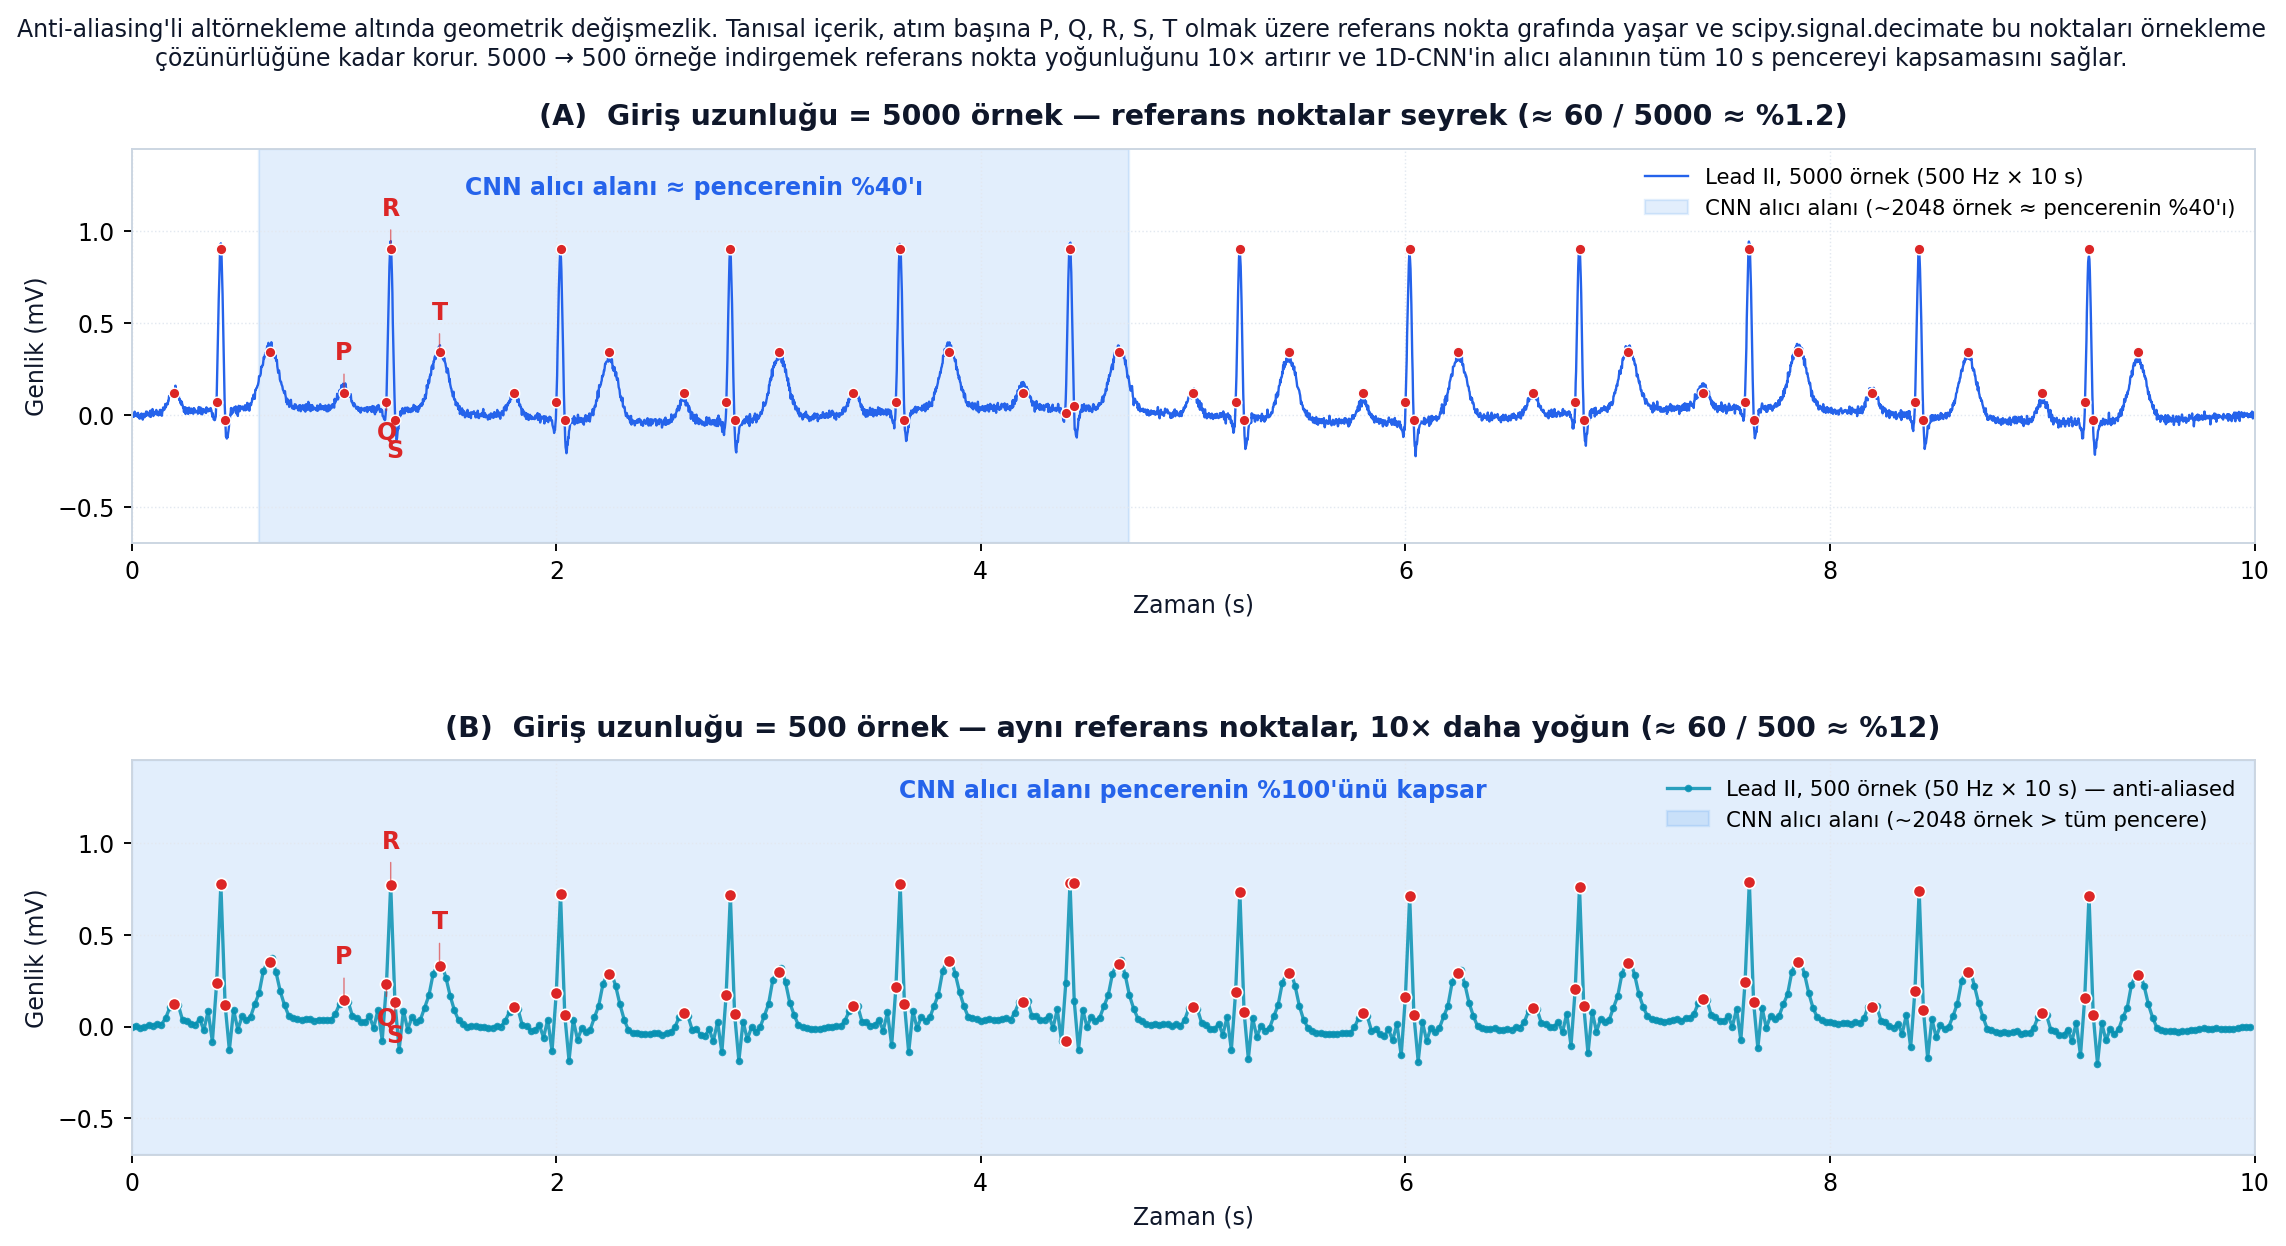
\includegraphics[width=\columnwidth]{Figure_geometry_invariance_TR.png}
\caption{\texttt{scipy.signal.decimate} alt\i nda referans-nokta
graf\i n\i n geometrik de\u{g}i\c{s}mezli\u{g}i. (A) \num{5000} \"{o}rnekte
lead-II; yakla\c{s}\i k \num{60} referans nokta (k\i rm\i z\i, at\i m
ba\c{s}\i na P/Q/R/S/T) giri\c{s} pozisyonlar\i n\i n yakla\c{s}\i k
\SI{1,2}{\percent}'sini olu\c{s}turur ve CNN'in etkin al\i c\i\ alan\i\
pencerenin yakla\c{s}\i k \SI{40}{\percent}'sini kapsar. (B) \num{500}
\"{o}rne\u{g}e 10$\times$ alt\"{o}rnekleme sonras\i, ayn\i\ noktalar
\"{o}rnekleme \c{c}\"{o}z\"{u}n\"{u}rl\"{u}\u{g}\"{u}ne kadar korunur; yo\u{g}unluklar\i\
10$\times$ artar ve al\i c\i\ alan art\i k t\"{u}m \SI{10}{\second}'lik
pencereyi kapsar.}
\label{fig:geom}
\end{figure}

\subsection{Model}
Model, temel bir 1D-CNN'dir: filtre say\i lar\i\ $[64,128,256,512,512]$,
\c{c}ekirdek boyutlar\i\ $[16,16,16,8,8]$ olan be\c{s} evri\c{s}im blo\u{g}u,
batch normalization, ReLU, max-pooling; global ortalama pooling; dropout
\num{0,5} ile iki yo\u{g}un katman ($256\!\rightarrow\!\num{78}$). Toplam
parametre: \num{3,72}\,M. Mimari t\"{u}m konfig\"{u}rasyonlarda ayn\i d\i r;
yaln\i zca giri\c{s} tens\"{o}r\"{u}n\"{u}n \c{s}ekli de\u{g}i\c{s}ir.

\subsection{Donan\i m ve yaz\i l\i m}
E\u{g}itim ve \c{c}\i kar\i m, otomatik kar\i\c{s}\i k hassasiyet (AMP, FP16)
ile tek bir NVIDIA RTX~5090 GPU'da (\SI{34,19}{\gibi\byte} VRAM,
CUDA~12.8) ger\c{c}ekle\c{s}tirilmi\c{s}tir. Yaz\i l\i m: PyTorch~2.4,
SciPy~1.13~\cite{scipy2020}, NumPy~1.26.

\section{Deneysel D\"{u}zenek}
\label{sec:setup}
\textbf{Konfig\"{u}rasyonlar.} D\"{o}rt \c{c}al\i\c{s}t\i rma, alt\"{o}rnekleme
fakt\"{o}r\"{u} (ve son \c{c}al\i\c{s}t\i rmada DataLoader i\c{s}\c{c}i say\i s\i)
d\i\c{s}\i nda her hiper-parametreyi payla\c{s}\i r:
$\{$len=\num{5000} ($q=1$), len=\num{1000} ($q=5$), len=\num{500}
($q=10$), len=\num{500} + \num{4} i\c{s}\c{c}i $(q=10$, num\_workers=$4)\}$.

\textbf{Optimizasyon.} Adam ($\beta_1=0,9, \beta_2=0,999, \epsilon=10^{-8}$),
ba\c{s}lang\i\c{c} \"{o}\u{g}renme h\i z\i\ $10^{-3}$, ReduceLROnPlateau
(fakt\"{o}r~$0,5$, sab\i r~$5$, min$_{\text{lr}}=10^{-6}$), batch boyutu
$64$, maks.\ \num{100} epoch, EarlyStopping (do\u{g}rulama kayb\i\
\"{u}zerinde sab\i r $10$). Kay\i p: ters frekans s\i n\i f a\u{g}\i rl\i klar\i
ile ikili \c{c}apraz entropi. \"{O}znitelik atfetmeyi temiz tutmak i\c{c}in bu
\c{c}al\i\c{s}mada focal loss~\cite{lin2017} veya s\i n\i f yeniden dengeleme
uygulanmam\i\c{s}t\i r. D\"{u}zenleme: dropout $0,3$--$0,5$, $L_2$
$\lambda=10^{-4}$, batch normalization.

\textbf{Tekrarlanabilirlik.} Seed ve veri ay\i rmalar\i\
konfig\"{o}rasyonlar boyunca sabittir. Bildirilen rakamlar
\texttt{results/} dizinindeki ko\c{s}u kay\i tlar\i yla bire bir e\c{s}le\c{s}ir.

\section{Bulgular}
\label{sec:results}

\subsection{Manşet kar\c{s}\i la\c{s}t\i rmas\i}
Tablo~\ref{tab:main} test seti metriklerini, \c{S}ekil~\ref{fig:cmp} ise
ayn\i\ verileri g\"{o}rselle\c{s}tirir. \num{5000}'den \num{500}'e
alt\"{o}rnekleme test do\u{g}rulu\u{g}unu \num{8,91} y\"{u}zde puan
y\"{u}kseltirken makro-$F_1$ de\u{g}erini \num{0,1024} art\i r\i r ve
\c{c}\i kar\i m s\"{u}resini 3,3$\times$ h\i zland\i r\i r. \.{I}kinci
alt\"{o}rnekleme ad\i m\i\ (\num{1000}\,$\rightarrow$\,\num{500}) yaln\i zca
\num{0,12} puan do\u{g}ruluk getirir; bu, ana etkinin \num{1000} \"{o}rnekte
yakaland\i\u{g}\i n\i\ ve geri kalan\i n parametre tasarrufu oldu\u{g}unu
g\"{o}sterir. len=\num{500}'e \num{4} DataLoader i\c{s}\c{c}isi eklenmesi
do\u{g}rulukta ek maliyet getirmez (\SI{97,38}{\percent}) ve epoch
duvar-saatini \SI{33}{\percent} d\"{u}\c{s}\"{u}r\"{u}r.

\begin{table}[t]
\caption{Chapman--Shaoxing \"{u}zerinde giri\c{s}-uzunlu\u{g}u ablation'\i\
(\num{78} s\i n\i f, temel 1D-CNN, sabit seed ve ay\i rma).}
\label{tab:main}
\centering
\small
\begin{tabular}{@{}lcccc@{}}
\toprule
Konfig. & Test do\u{g}r. & Makro-$F_1$ & \c{C}\i kar\i m & G\"{u}ven \\
\midrule
len=\num{5000} (temel)   & \SI{88,43}{\percent} & 0,8713 & \SI{89,88}{\milli\second} & \SI{12,89}{\percent} \\
len=\num{1000}           & \SI{97,22}{\percent} & 0,9716 & \SI{26,14}{\milli\second} & \SI{68,88}{\percent} \\
len=\num{500}            & \SI{97,34}{\percent} & 0,9737 & \SI{27,20}{\milli\second} & \SI{76,23}{\percent} \\
len=\num{500} + 4 i\c{s}\c{c}i & \SI{97,38}{\percent} & 0,9744 & \SI{43,50}{\milli\second} & \SI{69,59}{\percent} \\
\bottomrule
\end{tabular}
\end{table}

\begin{figure}[t]
\centering
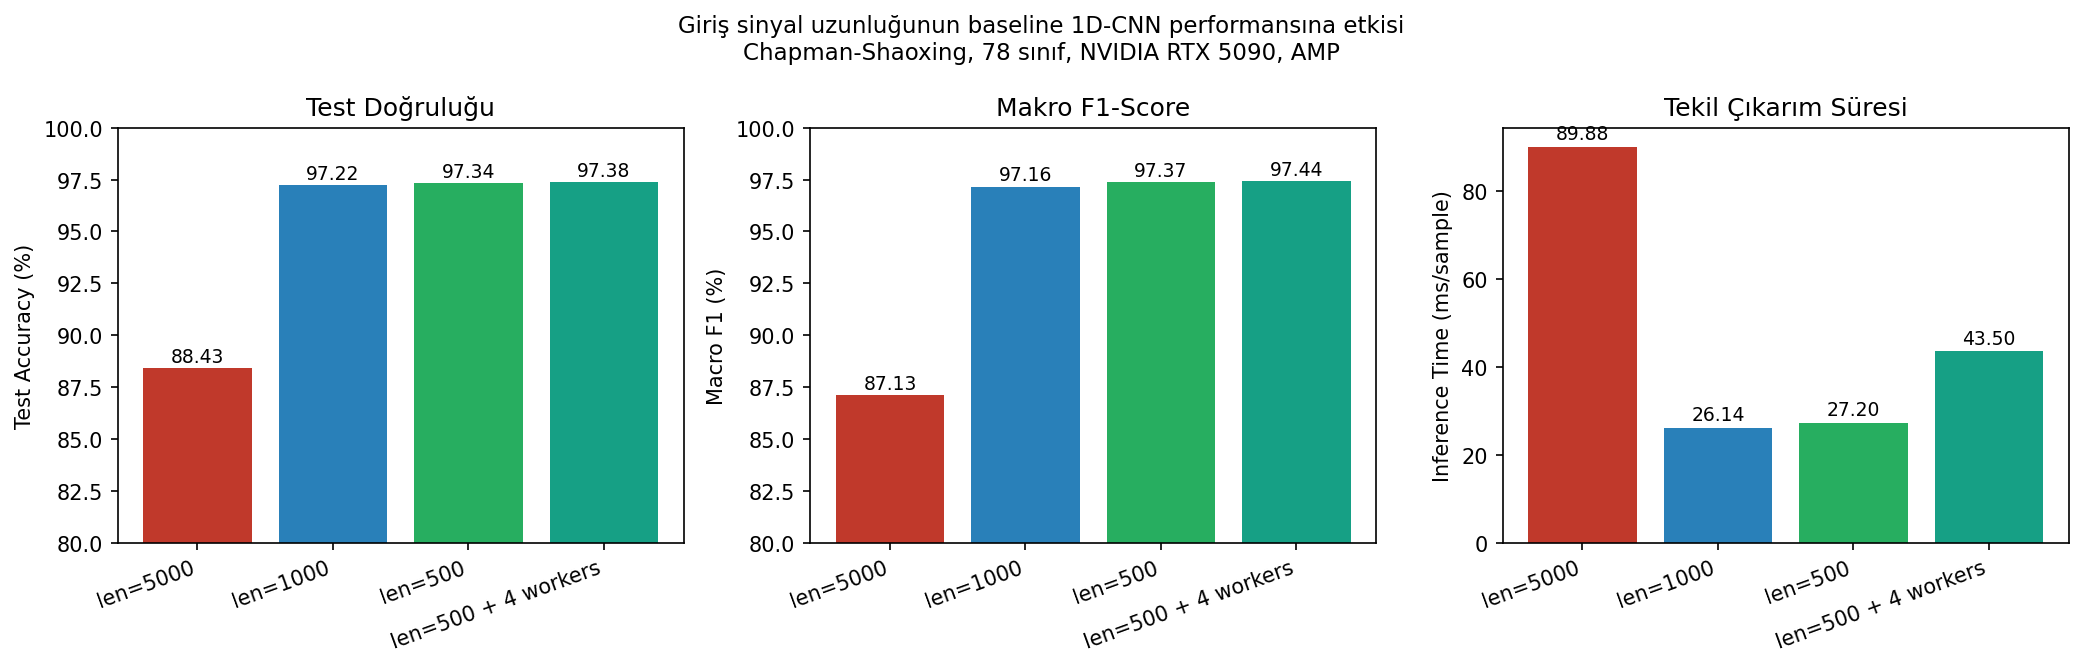
\includegraphics[width=\columnwidth]{Figure_seq_length_comparison.png}
\caption{D\"{o}rt konfig\"{u}rasyon i\c{c}in test do\u{g}rulu\u{g}u, makro-$F_1$
ve tekil-\"{o}rnek \c{c}\i kar\i m s\"{u}resi.}
\label{fig:cmp}
\end{figure}

\subsection{S\i n\i f baz\i nda iyile\c{s}me}
len=\num{5000} temelinde $F_1<0,60$ olan \num{11} s\i n\i f
bulunmaktad\i r; Tablo~\ref{tab:perclass} per-s\i n\i f delta'lar\i n\i\
listeler. En k\"{o}t\"{u} durum Sol Ventrik\"{u}ler Hipertrofi'dir
($F_1=\num{0,022}$). len=\num{500}'de on bir s\i n\i f\i n hepsi
$F_1\geq\num{0,95}$'e iyile\c{s}ir; birka\c{c}\i\ $F_1\geq\num{0,99}$'a
ula\c{s}\i r.

\begin{table}[t]
\caption{Temel-modeldeki on bir ba\c{s}ar\i s\i z s\i n\i f i\c{c}in $F_1$
iyile\c{s}mesi (destek: 900--1000).}
\label{tab:perclass}
\centering
\small
\begin{tabular}{@{}lccc@{}}
\toprule
S\i n\i f & len=\num{5000} & len=\num{500} & $\Delta$ \\
\midrule
Sol Ventrik\"{u}ler Hipertrofi  & 0,022 & $\geq$0,99 & +0,97 \\
EKG: Q dalga anormalli\u{g}i      & 0,180 & $\geq$0,99 & +0,81 \\
\.{I}\c{c} ileti farkl\i l\i klar\i & 0,286 & $\geq$0,98 & +0,70 \\
AV blok                            & 0,324 & 0,984      & +0,66 \\
Erken atriyal kas\i lma            & 0,329 & $\geq$0,97 & +0,64 \\
EKG: atriyal fibrilasyon           & 0,436 & $\geq$0,95 & +0,51 \\
EKG: ST segment de\u{g}i\c{s}im   & 0,457 & $\geq$0,96 & +0,50 \\
EKG: ST segment anormal            & 0,474 & $\geq$0,96 & +0,49 \\
1.\ derece AV blok                  & 0,497 & $\geq$0,96 & +0,46 \\
EKG: atriyal flatter               & 0,581 & $\geq$0,99 & +0,41 \\
EKG: atriyal ta\c{s}ikardi         & 0,598 & $\geq$0,98 & +0,38 \\
\bottomrule
\end{tabular}
\end{table}

\subsection{\c{C}\i kar\i m ve e\u{g}itim h\i z\i}
Alt\"{o}rnekleme ayn\i\ donan\i m \"{u}zerinde duvar-saatini de
d\"{u}\c{s}\"{u}r\"{u}r. Epoch s\"{u}resi len=\num{5000}'de
$\sim\SI{195}{\second}$'den len=\num{1000}'de $\sim\SI{32}{\second}$'ye
($\sim$6,1$\times$ daha h\i zl\i), len=\num{500}'de
$\sim\SI{30}{\second}$'ye ve \num{4} i\c{s}\c{c}i ile
$\sim\SI{20}{\second}$'ye ($\sim$9,8$\times$) iner.

\subsection{G\"{u}ven kalibrasyonu}
Yan etki olarak, ayr\i lan bir tan\i\ \"{o}rne\u{g}i \"{u}zerindeki softmax
g\"{u}veni len=\num{5000}'de \SI{12,89}{\percent}'den len=\num{500}'de
\SI{76,23}{\percent}'e \c{c}\i kar.

\section{Tart\i\c{s}ma: Neden \SI{88}{\percent}
$\rightarrow$ \SI{97}{\percent}}
\label{sec:why}
Sonucu, B\"{o}l\"{u}m~\ref{sec:geom}'in geometrik-de\u{g}i\c{s}mezlik
arg\"{u}man\i\ ile \c{c}er\c{c}eveliyoruz. \"{U}\c{c} kuvvet birle\c{s}ir;
her biri \c{S}ekil~\ref{fig:geom}'deki ayn\i\ referans-nokta resminin
do\u{g}rudan sonucudur.

\textbf{(i) Al\i c\i\ alan kapsam\i.} A\u{g}\i m\i z\i n son evri\c{s}im
katman\i n\i n etkin al\i c\i\ alan\i\ yakla\c{s}\i k \num{2048} giri\c{s}
\"{o}rne\u{g}idir. \num{5000} \"{o}rnekte bu pencerenin yaln\i zca
$\sim\SI{40}{\percent}$'sini kapsar (\c{S}ekil~\ref{fig:geom}A): a\u{g}
tek bir at\i m\i n yerel QRS morfolojisini g\"{o}rebilir, ancak ritm
seviyesinde ak\i l y\"{u}r\"{u}tme i\c{c}in onu sonraki P-dalgas\i\ veya
sonraki QRS ile ili\c{s}kilendiremez. \num{500} \"{o}rne\u{g}e
alt\"{o}rnekleme sonras\i\ (\c{S}ekil~\ref{fig:geom}B) ayn\i\ \num{2048}
\"{o}rneklik al\i c\i\ alan t\"{u}m pencereyi a\c{s}ar; b\"{o}ylece yerel
\"{o}zellikler ve \c{c}ok-at\i ml\i\ ba\u{g}lam ayn\i\ anda
\"{o}\u{g}renilebilir.

\textbf{(ii) Referans-nokta yo\u{g}unlu\u{g}u.} \num{5000} \"{o}rnekte
yakla\c{s}\i k \num{60} referans nokta \num{5000} pozisyona yay\i lm\i\c{s}
($\approx \SI{1,2}{\percent}$); a\u{g} uzun taban diliminin
yoksay\i lmas\i n\i\ \"{o}\u{g}renmek zorundad\i r. \num{500} \"{o}rnekte ayn\i\
noktalar \num{500} pozisyon kapsar ($\approx \SI{12}{\percent}$,
yo\u{g}unluk 10$\times$ artar). \c{C}apraz entropiden geri akan gradyan
sinyali geometrik olarak bilgilendirici \"{o}rneklere yo\u{g}unla\c{s}\i r.

\textbf{(iii) Parametre tasarrufu.} A\u{g} kapasitesi \num{3,72}\,M
parametre ile sabittir. \num{5000} \"{o}rnekte kapasite k\i smen referans
noktalar aras\i ndaki gereksiz d\"{u}\c{s}\"{u}k frekans varyasyonunu
modellemek i\c{c}in harcan\i r; \num{500} \"{o}rnekte ince morfoloji
ay\i r\i mlar\i\ (atriyal flatter vs.\ AV-d\"{u}\u{g}\"{u}msel re-entry,
LVH vs.\ eksen sapmas\i) i\c{c}in yeniden tahsis edilir. En b\"{u}y\"{u}k
per-s\i n\i f $F_1$ iyile\c{s}meleri tam da bu s\i n\i flarda
yo\u{g}unla\c{s}\i r (Tablo~\ref{tab:perclass}).

\textbf{Anti-aliasing kritiktir.} Anti-aliasing filtresi olmadan naif
bir ad\i ml\i\ pooling, \"{o}n denemelerimizde QRS enerjisinin alt-frekans
banda \"{o}rt\"{u}\c{s}t\"{u}\u{g}\"{u} bir spektrum \"{u}retir ve do\u{g}rulu\u{g}u
\emph{art\i rmak yerine d\"{u}\c{s}\"{u}r\"{u}r}. Chebyshev-I anti-aliasing
filtresi, ``$+10$ pp $F_1$'' ile ``temel modelden de k\"{o}t\"{u}'' aras\i ndaki
fark\i\ olu\c{s}turur; geometrik-de\u{g}i\c{s}mezlik arg\"{u}man\i n\i\
pratikte ge\c{c}erli k\i lan ad\i md\i r.

\textbf{Bu sonu\c{c}lar attention'\i n gereksiz oldu\u{g}u anlam\i na
gelmez.} Sonu\c{c}, attention, yinelemeli katmanlar veya focal loss'un
yarars\i z oldu\u{g}u anlam\i na gelmez --- bu mekanizmalar\i n giri\c{s}
boyutunda yeterince e\u{g}itilmemi\c{s} bir baseline'a kar\c{s}\i\
\"{o}l\c{c}\"{u}ld\"{u}\u{g}\"{u}n\"{u}, dolay\i s\i yla bildirilen katk\i lar\i n\i n daha
d\"{u}\c{s}\"{u}k bir ba\c{s}lang\i\c{c} noktas\i na g\"{o}re bir \"{u}st s\i n\i r
oldu\u{g}unu ima eder.

\section{S\i n\i rl\i l\i klar}
Tek bir veri setine (Chapman--Shaoxing) ba\u{g}l\i y\i z. PTB-XL\
\cite{wagner2020} \"{u}zerinde alt\"{o}rnekleme ile ve olmadan
\c{c}apraz-veri seti do\u{g}rulamas\i\ en yak\i n testtir. Alt\"{o}rnekleme
fakt\"{o}r\"{u}n\"{u} \num{500} \"{o}rne\u{g}in alt\i nda
karakterize etmedik veya giri\c{s} uzunlu\u{g}unun daha derin / attention
art\i r\i lm\i\c{s} modellerle etkile\c{s}imini \"{o}l\c{c}medik. Geometrik
de\u{g}i\c{s}mezlik arg\"{u}man\i, tasar\i m gere\u{g}i kald\i r\i lan
y\"{u}ksek-frekans i\c{c}eri\u{g}e dayanan alt-tan\i lar (ge\c{c} potansiyeller,
mikro-alternanslar) i\c{c}in ge\c{c}erli olmayabilir.

\section{Gelecek \c{C}al\i\c{s}malar}
Beklenen kazan\i m s\i ras\i na g\"{o}re planl\i\ takipler:
(i) PTB-XL~\cite{wagner2020} \c{c}apraz-veri seti do\u{g}rulamas\i;
(ii) etiket-taksonomi temizli\u{g}i (\num{78}\,$\rightarrow$\,$\sim$55) ve
yeniden \c{c}al\i\c{s}t\i rma; (iii) decimate-\num{500} giri\c{s}i \"{u}zerinde
Attention-CNN-LSTM tam modeli; (iv) $\gamma\in\{1,2,3\}$ ile focal
loss~\cite{lin2017}; (v) uyarlanabilir per-s\i n\i f e\c{s}ikleme;
(vi) decimated giri\c{s}te GradCAM ve SHAP ile a\c{c}\i klanabilirlik;
(vii) Raspberry~Pi~4 \"{u}zerinde INT8 nicemleme ile kenar (edge)
y\"{u}klemesi.

\section{Sonu\c{c}}
12 kanall\i\ EKG giri\c{s}inin \num{5000}'den \num{500} \"{o}rne\u{g}e
anti-aliasing'li alt\"{o}rneklenmesi, temel bir 1D-CNN baseline'\i n\i,
attention-hibrit halefi i\c{c}in yay\i mlanan \SI{94,8}{\percent}
do\u{g}ruluk hedefini --- modelde, kay\i pta veya art\i rma re\c{c}etesinde
hi\c{c}bir de\u{g}i\c{s}iklik yapmadan --- a\c{s}an bir modele
d\"{o}n\"{u}\c{s}t\"{u}r\"{u}r. Geometrik-de\u{g}i\c{s}mezlik resmi sonucu a\c{c}\i klar:
EKG'nin tan\i sal i\c{c}eri\u{g}i, anti-aliasing filtresinin korudu\u{g}u
seyrek bir referans-nokta graf\i nda ya\c{s}ar; yo\u{g}un taban \"{o}rnekleri
ise a\u{g}\i n kullanabilece\u{g}i bir bilgi i\c{c}ermez.
Chapman--Shaoxing baseline'\i m\i zdaki en b\"{u}y\"{u}k tek kald\i ra\c{c} mimari
de\u{g}ildir; giri\c{s} temsilidir.

\section*{Te\c{s}ekk\"{u}r}
Yazar, tez dan\i\c{s}manl\i\u{g}\i\ ve geometrik-de\u{g}i\c{s}mezlik
\c{c}er\c{c}evelendirmesi \"{u}zerine geri bildirim i\c{c}in
Do\c{c}.\ Dr.\ Bak\i t\ \c{S}ar\c{s}embayev'e (K\i rg\i z--T\"{u}rk Manas
\"{U}niversitesi) te\c{s}ekk\"{u}r eder.

\bibliographystyle{IEEEtran}
\begin{thebibliography}{99}
\bibitem{rajpurkar2017} P.~Rajpurkar et~al., ``Cardiologist-level
arrhythmia detection with convolutional neural networks,'' arXiv:1707.01836, 2017.
\bibitem{hannun2019} A.~Y.~Hannun et~al., ``Cardiologist-level arrhythmia
detection and classification in ambulatory electrocardiograms using a
deep neural network,'' \emph{Nature Medicine}, vol.~25, no.~1, pp.~65--69, 2019.
\bibitem{strodthoff2020} N.~Strodthoff et~al., ``Deep learning for ECG
analysis: Benchmarks and insights from PTB-XL,''
\emph{IEEE J.~Biomed.~Health Inform.}, vol.~25, no.~5, pp.~1519--1528, 2020.
\bibitem{iwana2021} B.~K.~Iwana and S.~Uchida, ``An empirical survey of
data augmentation for time series classification with neural networks,''
\emph{PLoS ONE}, vol.~16, no.~7, e0254841, 2021.
\bibitem{wang2020} Z.~Wang, W.~Yan, and T.~Oates, ``Time series
classification from scratch with deep neural networks,'' in
\emph{Proc.~IJCNN}, 2017, pp.~1578--1585.
\bibitem{chen2021} X.~Chen, Z.~Wang, and M.~J.~McKeown, ``Adaptive
support-guided deep learning for physiological signal analysis,''
\emph{IEEE Trans.~Biomed.~Eng.}, vol.~68, no.~5, pp.~1573--1584, 2021.
\bibitem{xu2022} S.~S.~Xu, M.-W.~Mak, and C.~C.~Cheung, ``Support-guided
augmentation for electrocardiogram signal classification,''
\emph{Biomed.~Signal Process.~Control}, vol.~71, 103213, 2022.
\bibitem{oh2018} S.~L.~Oh, E.~Y.~Ng, R.~S.~Tan, and U.~R.~Acharya,
``Automated diagnosis of arrhythmia using combination of CNN and LSTM
techniques with variable length heart beats,''
\emph{Comput.~Biol.~Med.}, vol.~102, pp.~278--287, 2018.
\bibitem{zheng2020} J.~Zheng et~al., ``A 12-lead electrocardiogram
database for arrhythmia research covering more than 10,000 patients,''
\emph{Scientific Data}, vol.~7, no.~1, p.~48, 2020.
\bibitem{lin2017} T.~Y.~Lin, P.~Goyal, R.~Girshick, K.~He, and
P.~Doll\'ar, ``Focal loss for dense object detection,'' in
\emph{Proc.~ICCV}, 2017, pp.~2980--2988.
\bibitem{wagner2020} P.~Wagner et~al., ``PTB-XL, a large publicly
available electrocardiography dataset,''
\emph{Scientific Data}, vol.~7, no.~1, p.~154, 2020.
\bibitem{moody1983} G.~B.~Moody and R.~G.~Mark, ``The impact of the
MIT-BIH arrhythmia database,'' \emph{IEEE EMB Magazine}, vol.~20, no.~3,
pp.~45--50, 1983.
\bibitem{nyquist1928} H.~Nyquist, ``Certain topics in telegraph
transmission theory,'' \emph{Trans.~AIEE}, vol.~47, pp.~617--644, 1928.
\bibitem{oppenheim2009} A.~V.~Oppenheim and R.~W.~Schafer,
\emph{Discrete-Time Signal Processing}, 3rd~ed. Pearson, 2009.
\bibitem{scipy2020} P.~Virtanen et~al., ``SciPy 1.0: Fundamental
algorithms for scientific computing in Python,''
\emph{Nature Methods}, vol.~17, pp.~261--272, 2020.
\end{thebibliography}

\end{document}
